\documentclass{article}
\usepackage[utf8]{inputenc}
\usepackage{blindtext}
\usepackage{enumitem}
\usepackage{graphicx}
\usepackage{hyperref}
\usepackage{titletoc}
\usepackage{float} 
\usepackage{fullpage}
\usepackage[color]{vdmlisting}
\usepackage{longtable}
\graphicspath{ {images/} }

\hypersetup{colorlinks=true,
urlcolor=blue,
linkcolor=black}

\title{ \begin{center}
					
\includegraphics[scale=0.6]{./images/FEUPlogo}
				\end{center}
				\textbf{FashionShow}}
\author{Miguel Lira Barbeitos Luís - up201405324\\
		Miriam Cristiana Meireles Campos Gonçalves - up201403441\\
		Paulo Sérgio Silva Babo - up201404022}
\date{03 Janeiro, 2018}
\begin{document}

\begin{titlepage}
	\centering
	
\includegraphics[width=1\textwidth]{./images/FEUPlogo}\par\vspace{1cm}
	{\huge\bfseries Fashion Show \par}
	\vspace{2cm}
	{\scshape\Large Relatório Final\par}
	\vspace{1.5cm}
	{\large\bfseries Métodos Formais em Engenharia de Software\par}
	\vspace{0.7cm}
	{\scshape\normalsize  Mestrado Integrado em Engenharia Informática e Computação \par}
	\vspace{1.5cm}
	{\Large\itshape Grupo\textunderscore04 Turma\textunderscore01 
	\par Miguel Lira Barbeitos Luís - up201405324 \par
	Miriam Cristiana Meireles Campos Gonçalves - up201403441 \par
	Paulo Sérgio Silva Babo - up201404022\par}

	\vfill
% Bottom of the page
	{\large \today\par}
\end{titlepage}
\thispagestyle{empty}

\newpage

\tableofcontents

\newpage

\section{Descrição Informal do Sistema e Lista de Requisitos}
\subsection{Descrição Informal do Sistema}
\subsection{Lista de Requisitos}

\section{Modelo UML}
\subsection{Modelo de Casos de Uso}
\subsection{Diagrama de Classes}
\begin{figure}[H]
\centering
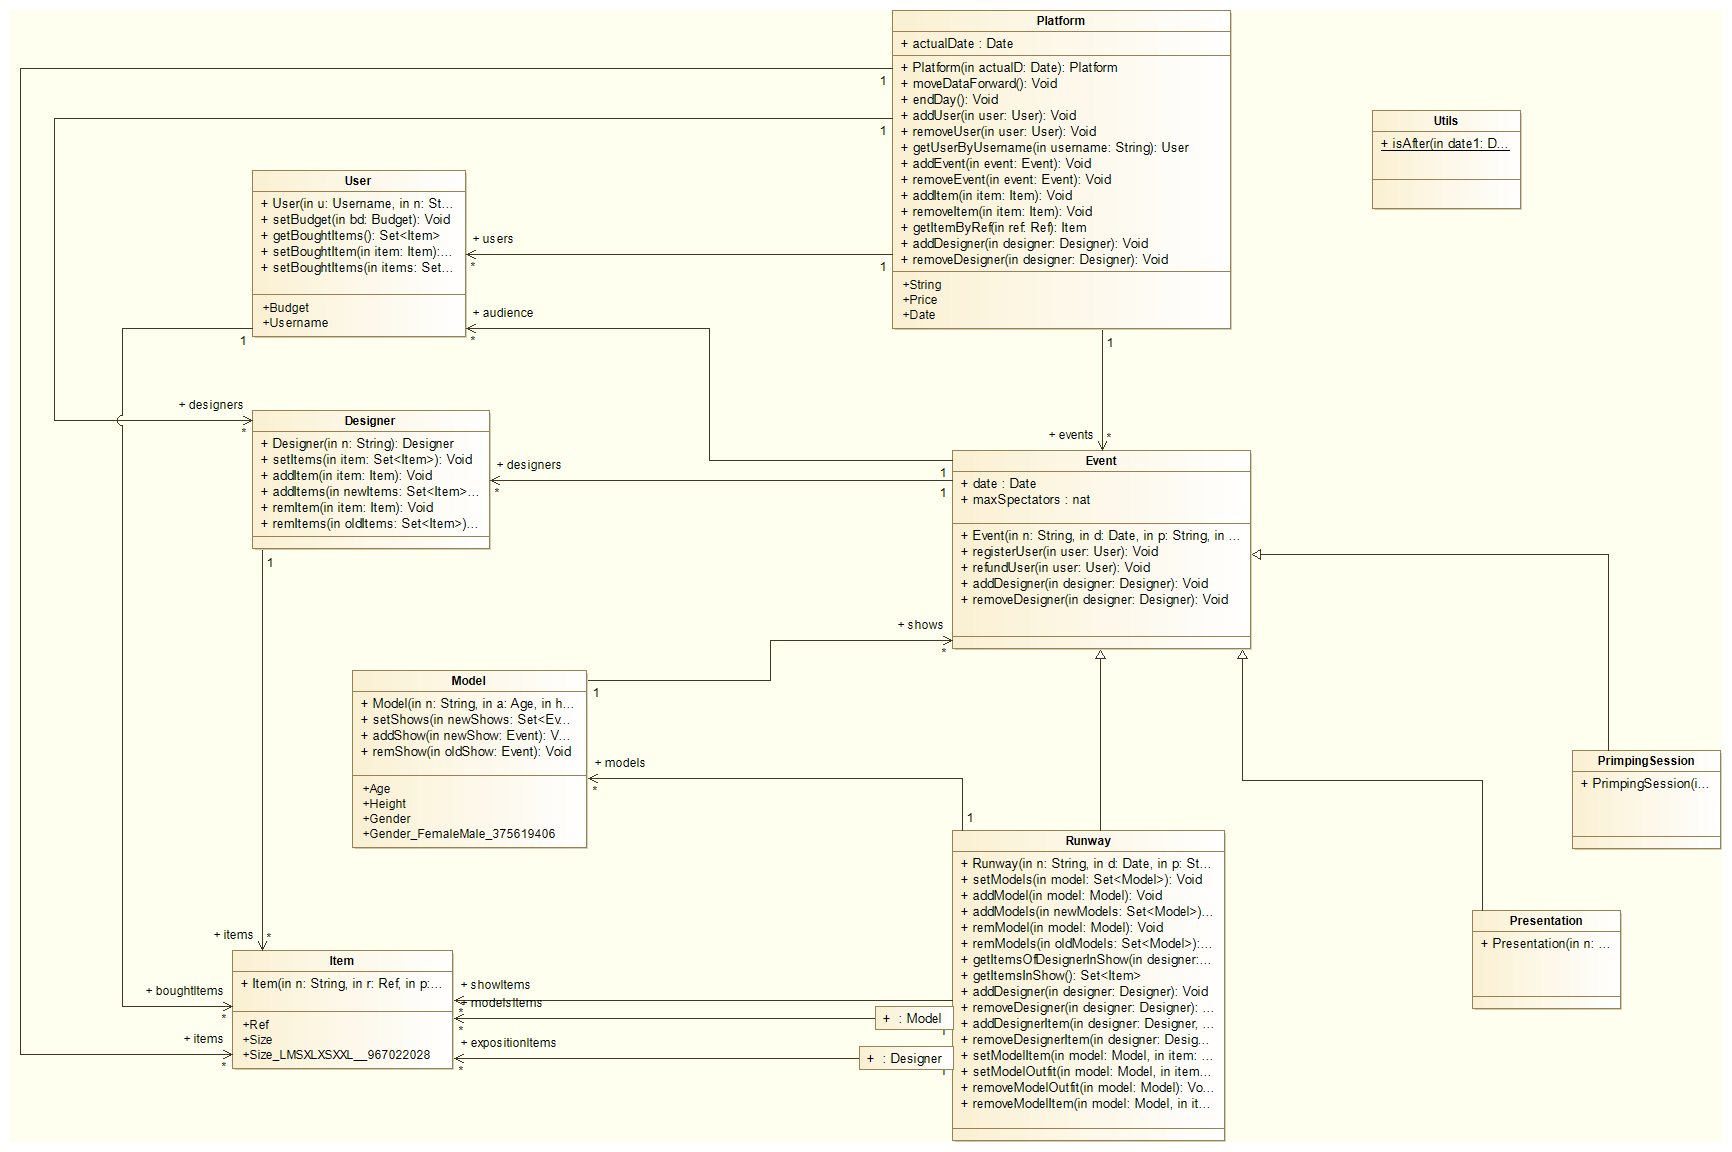
\includegraphics[width=160mm,height=150mm]{./images/class_diagram.png}
\caption{Diagrama de classes}
\label{fig:method}
\end{figure}
		
\section{Modelo Formal VDM++}
\subsection{Class Platform}

\subsection{Class User}
\subsection{Class Event}
\subsection{Class PrimpingSession}
\subsection{Class Presentation}
\subsection{Class Runway}
\subsection{Class Model}
\subsection{Class Designer}
\begin{vdmpp}[breaklines=true]
/**
* Esta classe representa um Designer bem como os itens que dispoe para os shows
*/
class Designer
types

instance variables
  /**
  * nome do designer
  */
  public name: Platform`String;
  /**
  * itens dos quais o designer dispoe
  */
  public items: set of Item;
values
 
operations
 /**
 * Designer construtor
 * 
 * @param n nome de um designer
 */
(*@
\label{Designer:24}
@*)
 public Designer: Platform`String ==> Designer 
  Designer(n) == (
   name := n;
   items := {};
   return self;
 );
 
 /**
 * Insercao de um conjunto de itens nos itens de um designer
 * 
 * @param item corresponde aos itens a serem inseridos
 */
(*@
\label{setItems:36}
@*)
 public setItems: set of Item ==> ()
   setItems(item) == 
    items := item;
    
 /**
 * Insercao de um item no conjunto de itens de um designer
 * 
 * @param item corresponde ao item a ser inserido
 */
(*@
\label{addItem:45}
@*)
 public addItem: Item ==> ()
  addItem(item) == (
     items := items union {item}
  )
 pre item not in set items
 post item in set items;
 
 /**
 * Insercao de um conjunto de itens nos itens de um designer
 * 
 * @param newItems corresponde aos itens a serem inseridos
 */
(*@
\label{addItems:57}
@*)
 public addItems: set of Item ==> ()
  addItems(newItems) == (
    for all i in set newItems do (
      items := items union {i};
    )
   )
 pre (not newItems subset items) and newItems <> items
 post newItems subset items;
   
  /**
 * Remocao de um item do conjunto de itens de um designer
 * 
 * @param item corresponde ao item a ser removido
 */
(*@
\label{remItem:71}
@*)
 public remItem: Item ==> ()
  remItem(item) ==
      items := items \ {item}
 pre items <> {} and item in set items
 post item not in set items;
  
 /**
 * Remocao de um conjunto de itens dos itens de um designer
 * 
 * @param oldItems corresponde aos itens a serem removidos
 */
(*@
\label{remItems:82}
@*)
 public remItems: set of Item ==> ()
  remItems(oldItems) ==
    for all i in set oldItems do (
      items := items \ {i}
    )
 pre items <> {} and (oldItems subset items)
 post not oldItems subset items;
  
functions

end Designer

\end{vdmpp}
\bigskip
\begin{longtable}{|l|r|r|r|}
\hline
Function or operation & Line & Coverage & Calls \\
\hline
\hline
\hyperref[Designer:24]{Designer} & 24&100.0\% & 117 \\
\hline
\hyperref[addItem:45]{addItem} & 45&100.0\% & 3 \\
\hline
\hyperref[addItems:57]{addItems} & 57&100.0\% & 57 \\
\hline
\hyperref[remItem:71]{remItem} & 71&100.0\% & 3 \\
\hline
\hyperref[remItems:82]{remItems} & 82&100.0\% & 3 \\
\hline
\hyperref[setItems:36]{setItems} & 36&100.0\% & 12 \\
\hline
\hline
Designer.vdmpp & & 100.0\% & 195 \\
\hline
\end{longtable}


\subsection{Class Item}
\subsection{Class Utils}

\section{Modelo de Validação}
\subsection{Class Test}

\section{Modelo de Verificação}

\section{Geração de código}

\section{Conclusões}
\section{Referências}
\subsection{Bibliografia}
\noindent
(1) Peter Gorm Larsen, Kenneth Lausdahl, Nick Battle, John Fitzgerald, Sune Wolff, Shin Sahara, Marcel Verhoef, Peter W. V. Tran-Jørgensen, Tomohiro Oda, Paul Chisholm, Overture "VDM-10 Language Manual"\\

\noindent
(2) Peter Gorm Larsen, John Fitzgerald, Sune Wolff, Nick Battle, Kenneth Lausdahl, Augusto Ribeiro, Kenneth Pierce, Victor Bandur, "Tutorial for Overture/VDM++"\\

\noindent
(3) Sarit Kraus, Katia Sycara, Amir Evenchik, "Reaching agreements through argumentation: a logical model and implementation"\\

\noindent
(4) Peter Gorm Larsen, Kenneth Lausdahl, Peter Jørgensen, Joey Coleman, Sune Wolff and Luís Diogo Couto Aarhus University, Department of Engineering Finlandsgade 22, DK-8000 Aarhus C, Denmark, "Overture VDM-10 Tool Support: User Guide"\\
\subsection{Software}

Eclipse \\
\vspace{3mm}\url{http://www.eclipse.org/} \\
Overture \\
\vspace{3mm}\url{http://overturetool.org/} \\
Modelio \\
\vspace{3mm}\url{https://www.modelio.org/} \\
\end{document}